
\section{Bedienoberfläche}

Hier sollen die Skizzen/Prototypen von Bedienoberflächen dargestellt werden, als auch die Zusammenhänge zwischen denen (wie gelingt man von einem zu dem anderen Fenster/Ansicht).\footnote{Bevor Sie mit den Skizzen anfangen, überlegen Sie sich, welche virtuelle Räume im System zu haben sind und dann halte Sie die Namen der GUI-Fenstern mit diesen konsistent.}

\newcounter{gui}\setcounter{gui}{10}


\begin{description}[leftmargin=5em, style=sameline]	
	\begin{lhp}{gui}{GUI}{gui:beispiel}
		\item[Name:] Zusammenhang
		\item[Beschreibung:] Zusammenhangzwischen alle GUI-Elemente
		\item[Relevante Systemfunktionen:] Alle
		\item[Abbildungen:] \ref{gui:zsm}
	\end{lhp}
\end{description}

\begin{description}[leftmargin=5em, style=sameline]	
	\begin{lhp}{gui}{GUI}{gui:beispiel}
		\item[Name:] Vorraum-Interface
		\item[Beschreibung:] Interface für Anmeldung und Registrierung
		\item[Relevante Systemfunktionen:] \ref{funk:zugriff}
		\item[Abbildungen:] \ref{gui:vorraum}
	\end{lhp}
\end{description}

\begin{description}[leftmargin=5em, style=sameline]	
	\begin{lhp}{gui}{GUI}{gui:beispiel}
		\item[Name:] Anmeldung-Interface
		\item[Beschreibung:] Interface für die Anmeldung
		\item[Relevante Systemfunktionen:] \ref{funk:zugriff}
		\item[Abbildungen:] \ref{gui:anmeldung}
	\end{lhp}
\end{description}

\begin{description}[leftmargin=5em, style=sameline]	
	\begin{lhp}{gui}{GUI}{gui:beispiel}
		\item[Name:] Registrierung-Interface
		\item[Beschreibung:] Interface für die Registrierung
		\item[Relevante Systemfunktionen:] \ref{funk:zugriff}
		\item[Abbildungen:] \ref{gui:registrieren}
	\end{lhp}
\end{description}

\begin{description}[leftmargin=5em, style=sameline]	
	\begin{lhp}{gui}{GUI}{gui:beispiel}
		\item[Name:] Lobby-Interface
		\item[Beschreibung:] Interface für die Lobby mit Chat-Funktion und Bestenliste
		\item[Relevante Systemfunktionen:] \ref{funk:bestenliste}, \ref{funk:chat}
		\item[Abbildungen:] \ref{gui:lobby}
	\end{lhp}
\end{description}

\begin{description}[leftmargin=5em, style=sameline]	
	\begin{lhp}{gui}{GUI}{gui:beispiel}
		\item[Name:] Einstellung-Interface
		\item[Beschreibung:] Interface für die Einstellungen, wo man seine Kontodaten bearbeiten kann (und auch Lautstärke ändern, falls implementiert wird)
		\item[Relevante Systemfunktionen:] \ref{funk:zugriff}
		\item[Abbildungen:] \ref{gui:einstellung}
	\end{lhp}
\end{description}

\begin{description}[leftmargin=5em, style=sameline]	
	\begin{lhp}{gui}{GUI}{gui:beispiel}
		\item[Name:] Passwortänderung-Interface
		\item[Beschreibung:] Interface für die Passwortänderung
		\item[Relevante Systemfunktionen:] \ref{funk:zugriff}
		\item[Abbildungen:] \ref{gui:passwort}
	\end{lhp}
\end{description}

\begin{description}[leftmargin=5em, style=sameline]	
	\begin{lhp}{gui}{GUI}{gui:beispiel}
		\item[Name:] Kontolöschung-Interface
		\item[Beschreibung:] Interface für die Löschung des Kontos
		\item[Relevante Systemfunktionen:] \ref{funk:zugriff}
		\item[Abbildungen:] \ref{gui:konto}
	\end{lhp}
\end{description}

\begin{description}[leftmargin=5em, style=sameline]	
	\begin{lhp}{gui}{GUI}{gui:beispiel}
		\item[Name:] Raumerstellung-Interface
		\item[Beschreibung:] Interface für die Raumerstellung. Hier kann man die maximale Anzahl an Spieler, Name des Raums angeben. Man kann auch sich entscheiden ob er mit Bots spielen will.
		\item[Relevante Systemfunktionen:] \ref{funk:spielraum}
		\item[Abbildungen:] \ref{gui:erstellen}
	\end{lhp}
\end{description}

\begin{description}[leftmargin=5em, style=sameline]	
	\begin{lhp}{gui}{GUI}{gui:beispiel}
		\item[Name:] Spielraum-Interface
		\item[Beschreibung:] Interface für das Spielraum
		\item[Relevante Systemfunktionen:] \ref{funk:spielraum}
		\item[Abbildungen:] \ref{gui:raum}
	\end{lhp}
\end{description}

\begin{description}[leftmargin=5em, style=sameline]	
	\begin{lhp}{gui}{GUI}{gui:beispiel}
		\item[Name:] Spiel-Interface
		\item[Beschreibung:] Interface für das Spiel. Hier wird die Anzahl an Chips von alle Spielern gezeigt sowie die Anzahl an Chips im Pot. Der Pfeil zeigt wer zurzeit dran ist. Die Rangliste zeigt die Anzahl der Punkte von Spielern in diesem Spiel.
		\item[Relevante Systemfunktionen:] \ref{funk:bots}, \ref{funk:spielverw}
		\item[Abbildungen:] \ref{gui:spiel}
	\end{lhp}
\end{description}

\begin{description}[leftmargin=5em, style=sameline]	
	\begin{lhp}{gui}{GUI}{gui:beispiel}
		\item[Name:] Gewonnen-Interface
		\item[Beschreibung:] Fenster wird angezeigt, wenn das Spiel zum Ende ist
		\item[Relevante Systemfunktionen:] \ref{funk:spielverw}
		\item[Abbildungen:] \ref{gui:win}
	\end{lhp}
\end{description}

\begin{figure}
	\centering
	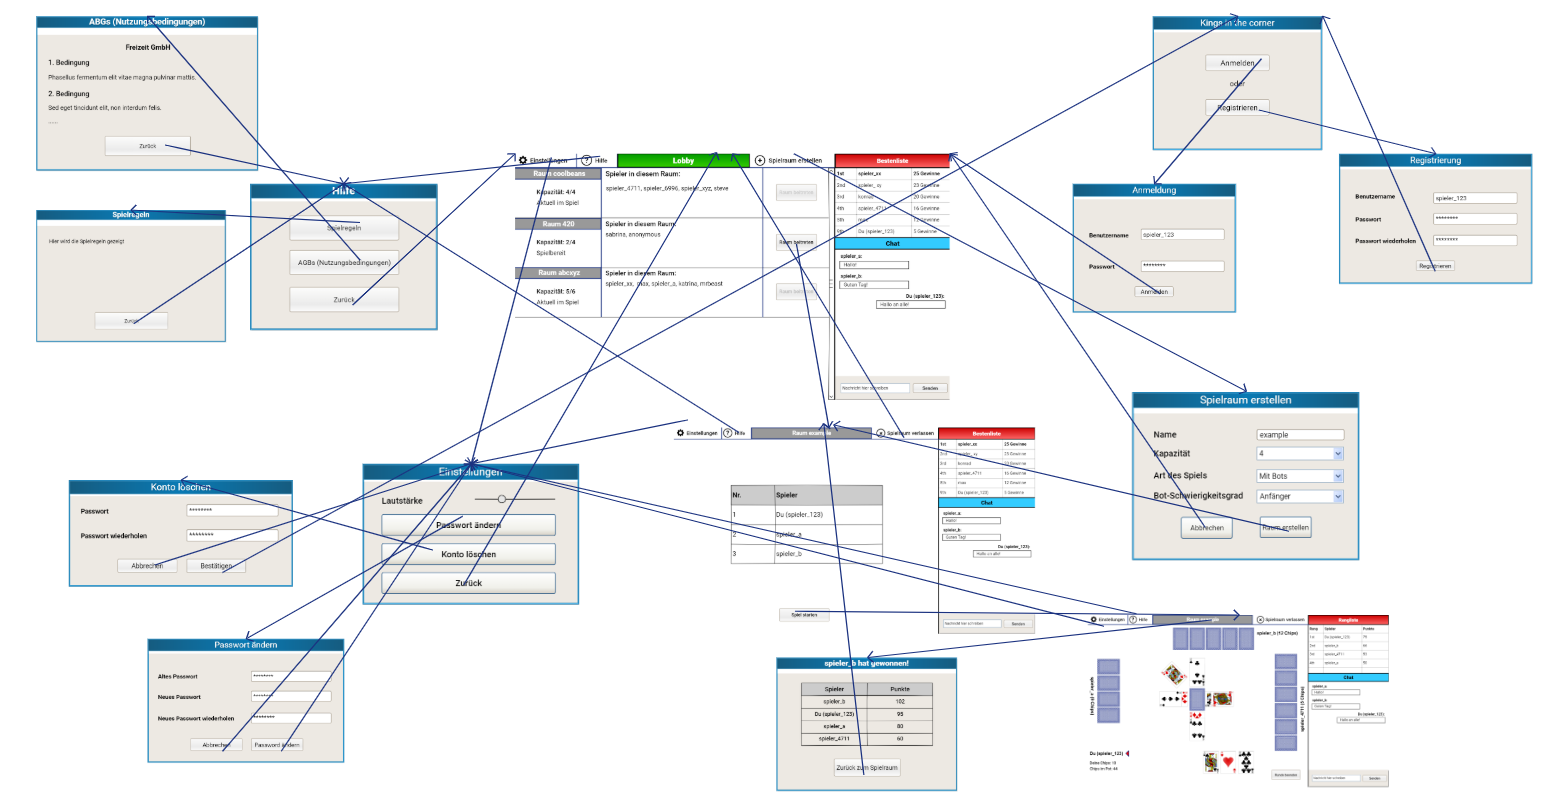
\includegraphics[width=0.9\textwidth]{SEP_Lasten_Pflichtenheft/img/GUI/zusammenhang.png}
	\caption{Zusammenhang zwischen alle GUI-Elemente}
	\label{gui:zsm}
\end{figure}

\begin{figure}
	\centering
	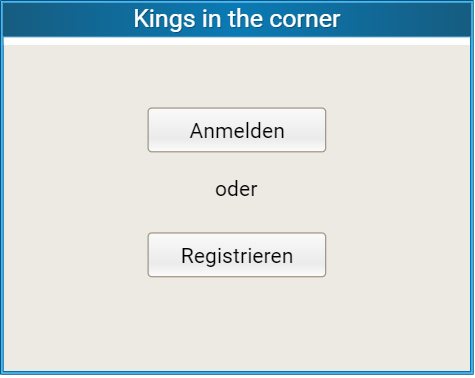
\includegraphics[width=0.9\textwidth]{SEP_Lasten_Pflichtenheft/img/GUI/anfangsfenster.png}
	\caption{Vorraum-Fenster}
	\label{gui:vorraum}
\end{figure}

\begin{figure}
	\centering
	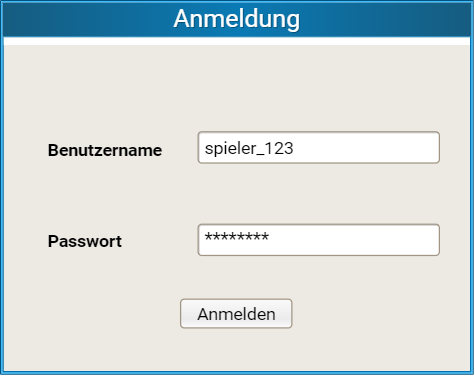
\includegraphics[width=0.9\textwidth]{SEP_Lasten_Pflichtenheft/img/GUI/anmelden.png}
	\caption{Anmeldung-Interface}
	\label{gui:anmeldung}
\end{figure}

\begin{figure}
	\centering
	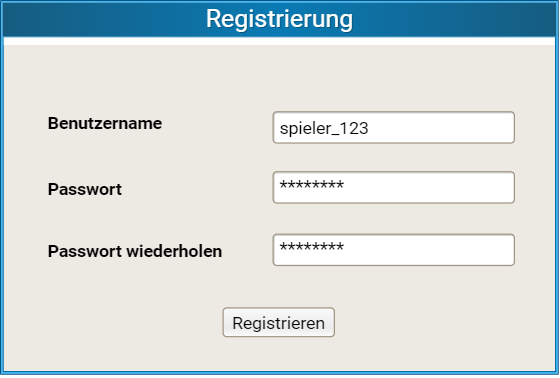
\includegraphics[width=0.9\textwidth]{SEP_Lasten_Pflichtenheft/img/GUI/registrieren.png}
	\caption{Registrierung-Interface}
	\label{gui:registrieren}
\end{figure}

\begin{figure}
	\centering
	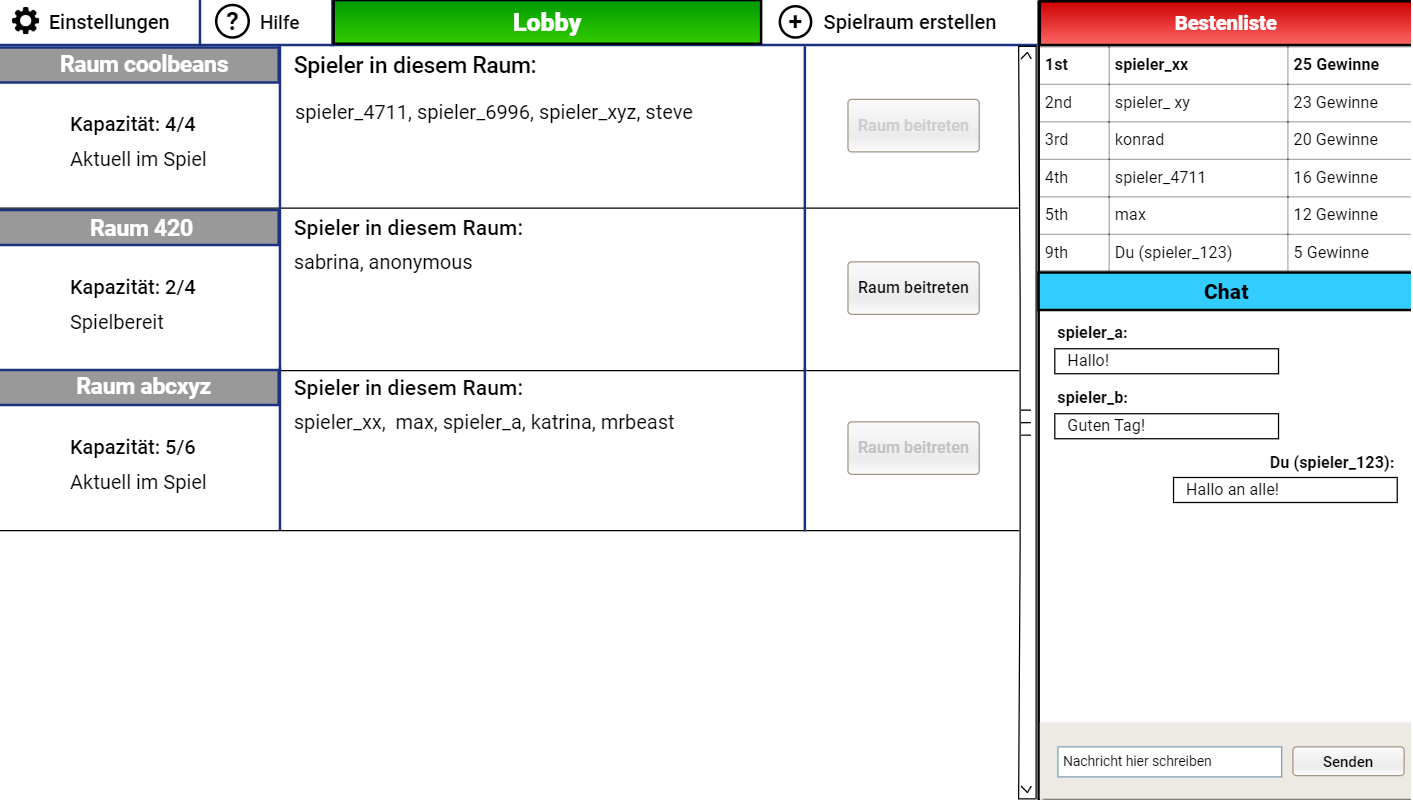
\includegraphics[width=0.9\textwidth]{SEP_Lasten_Pflichtenheft/img/GUI/lobby.png}
	\caption{Lobby-Interface mit Chatfunktion und Bestenliste}
	\label{gui:lobby}
\end{figure}

\begin{figure}
	\centering
	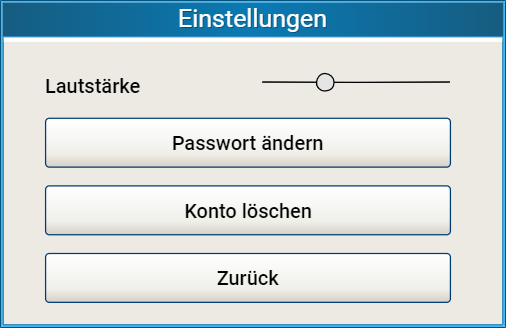
\includegraphics[width=0.9\textwidth]{SEP_Lasten_Pflichtenheft/img/GUI/einstellungen.png}
	\caption{Einstellungen-Interface mit Möglichkeit zur Passwortänderung sowie Kontolöschung (und auch Lautstärke falls implementiert wird)}
	\label{gui:einstellung}
\end{figure}

\begin{figure}
	\centering
	\includegraphics[width=0.9\textwidth]{SEP_Lasten_Pflichtenheft/img/GUI/passwortänderung.png}
	\caption{Passwortänderungsfenster}
	\label{gui:passwort}
\end{figure}

\begin{figure}
	\centering
	\includegraphics[width=0.9\textwidth]{SEP_Lasten_Pflichtenheft/img/GUI/kontolöschung.png}
	\caption{Kontolöschungsfenster}
	\label{gui:konto}
\end{figure}

\begin{figure}
	\centering
	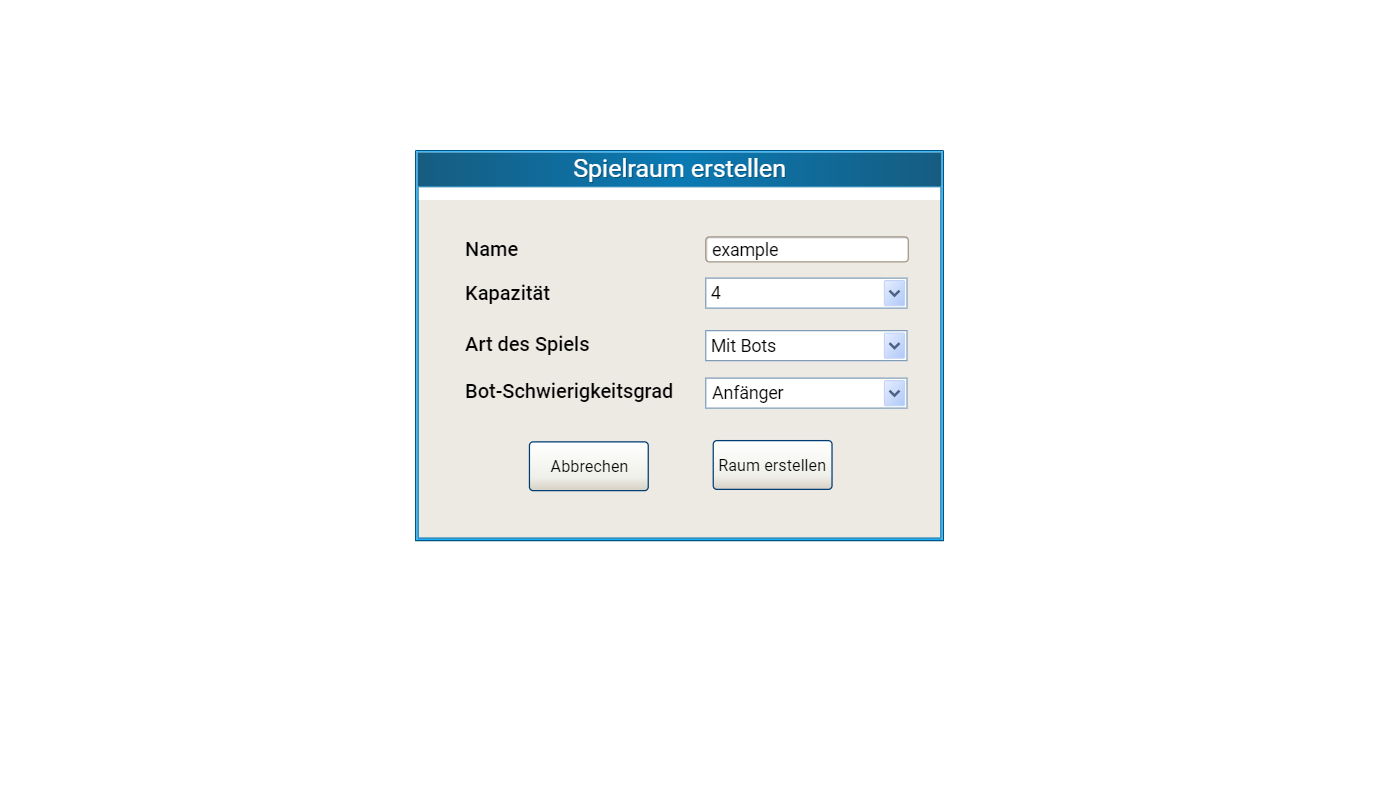
\includegraphics[width=0.9\textwidth]{SEP_Lasten_Pflichtenheft/img/GUI/raum_erstellen.png}
	\caption{Fenster zur Raumerstellung}
	\label{gui:erstellen}
\end{figure}

\begin{figure}
	\centering
	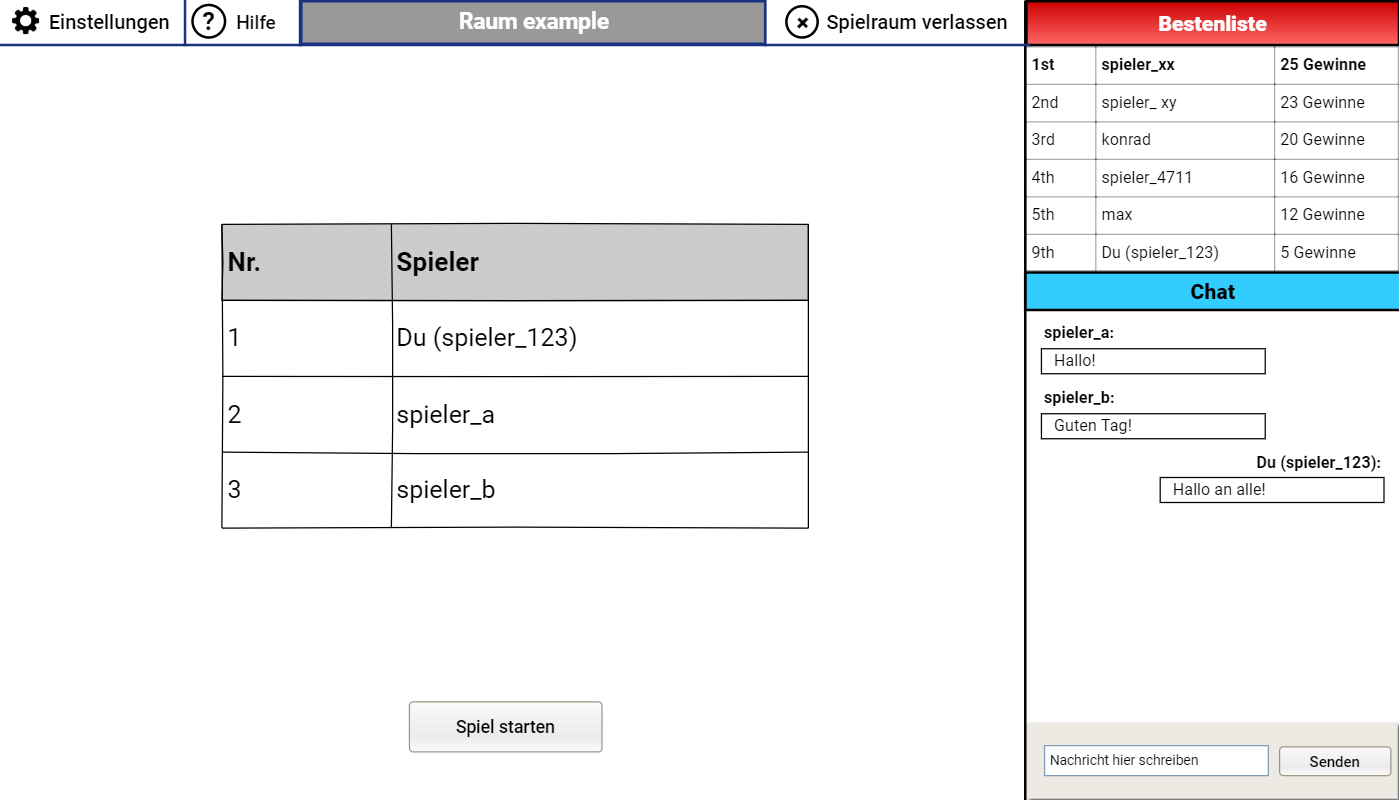
\includegraphics[width=0.9\textwidth]{SEP_Lasten_Pflichtenheft/img/GUI/spielraum.png}
	\caption{Spielraum-Interface}
	\label{gui:raum}
\end{figure}

\begin{figure}
	\centering
	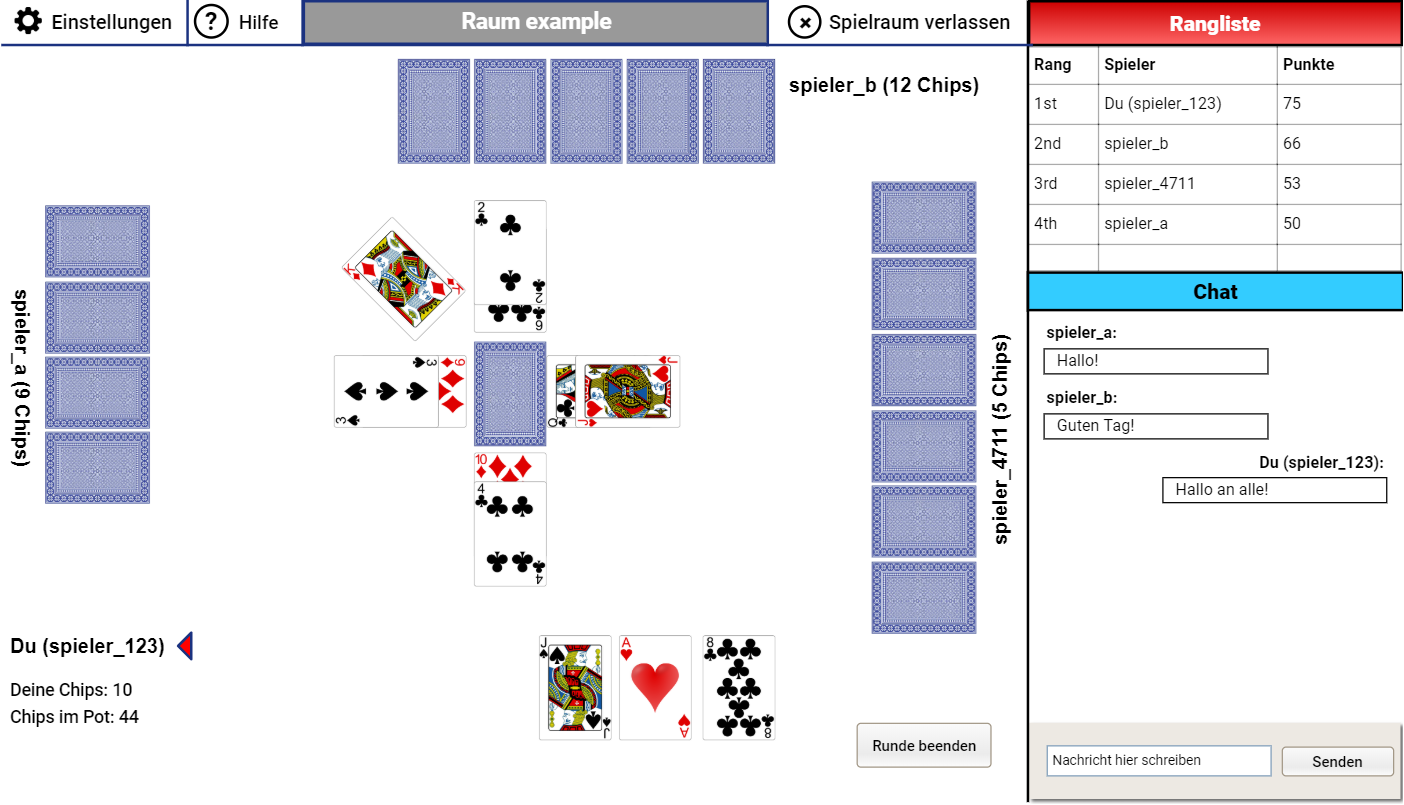
\includegraphics[width=0.9\textwidth]{SEP_Lasten_Pflichtenheft/img/GUI/spielen.png}
	\caption{Spiel-Interface}
	\label{gui:spiel}
\end{figure}

\begin{figure}
	\centering
	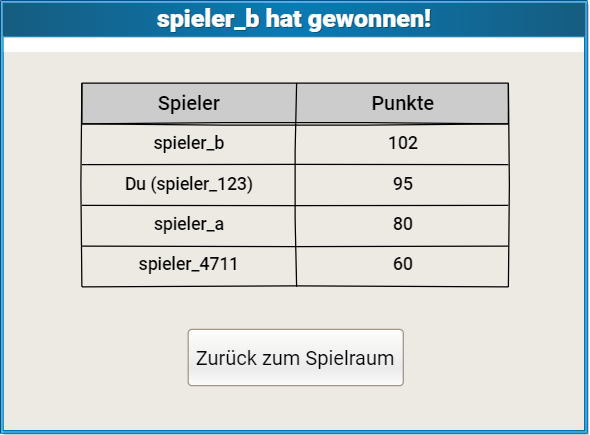
\includegraphics[width=0.9\textwidth]{SEP_Lasten_Pflichtenheft/img/GUI/gewonnen.png}
	\caption{Gewonnen-Fenster}
	\label{gui:win}
\end{figure}